\section{AudioMouth}
\label{sec:method}

We introduce AudioMouth, which generates mouth-related ARKit trajectories by making the articulatory structure of speech explicit on both sides of the mapping. We first organize long recordings into units where a phoneme and the motion it produces share one time span, then generate a fixed-schema coefficient sequence under phoneme-to-articulation grounding with supervision balanced across coefficient values, and finally refine the generator with a reward computed on the decoded motion. The formulation, the three stages, and inference are introduced as follows.

\begin{figure*}[t]
    \centering
    \vspace{-2mm}
    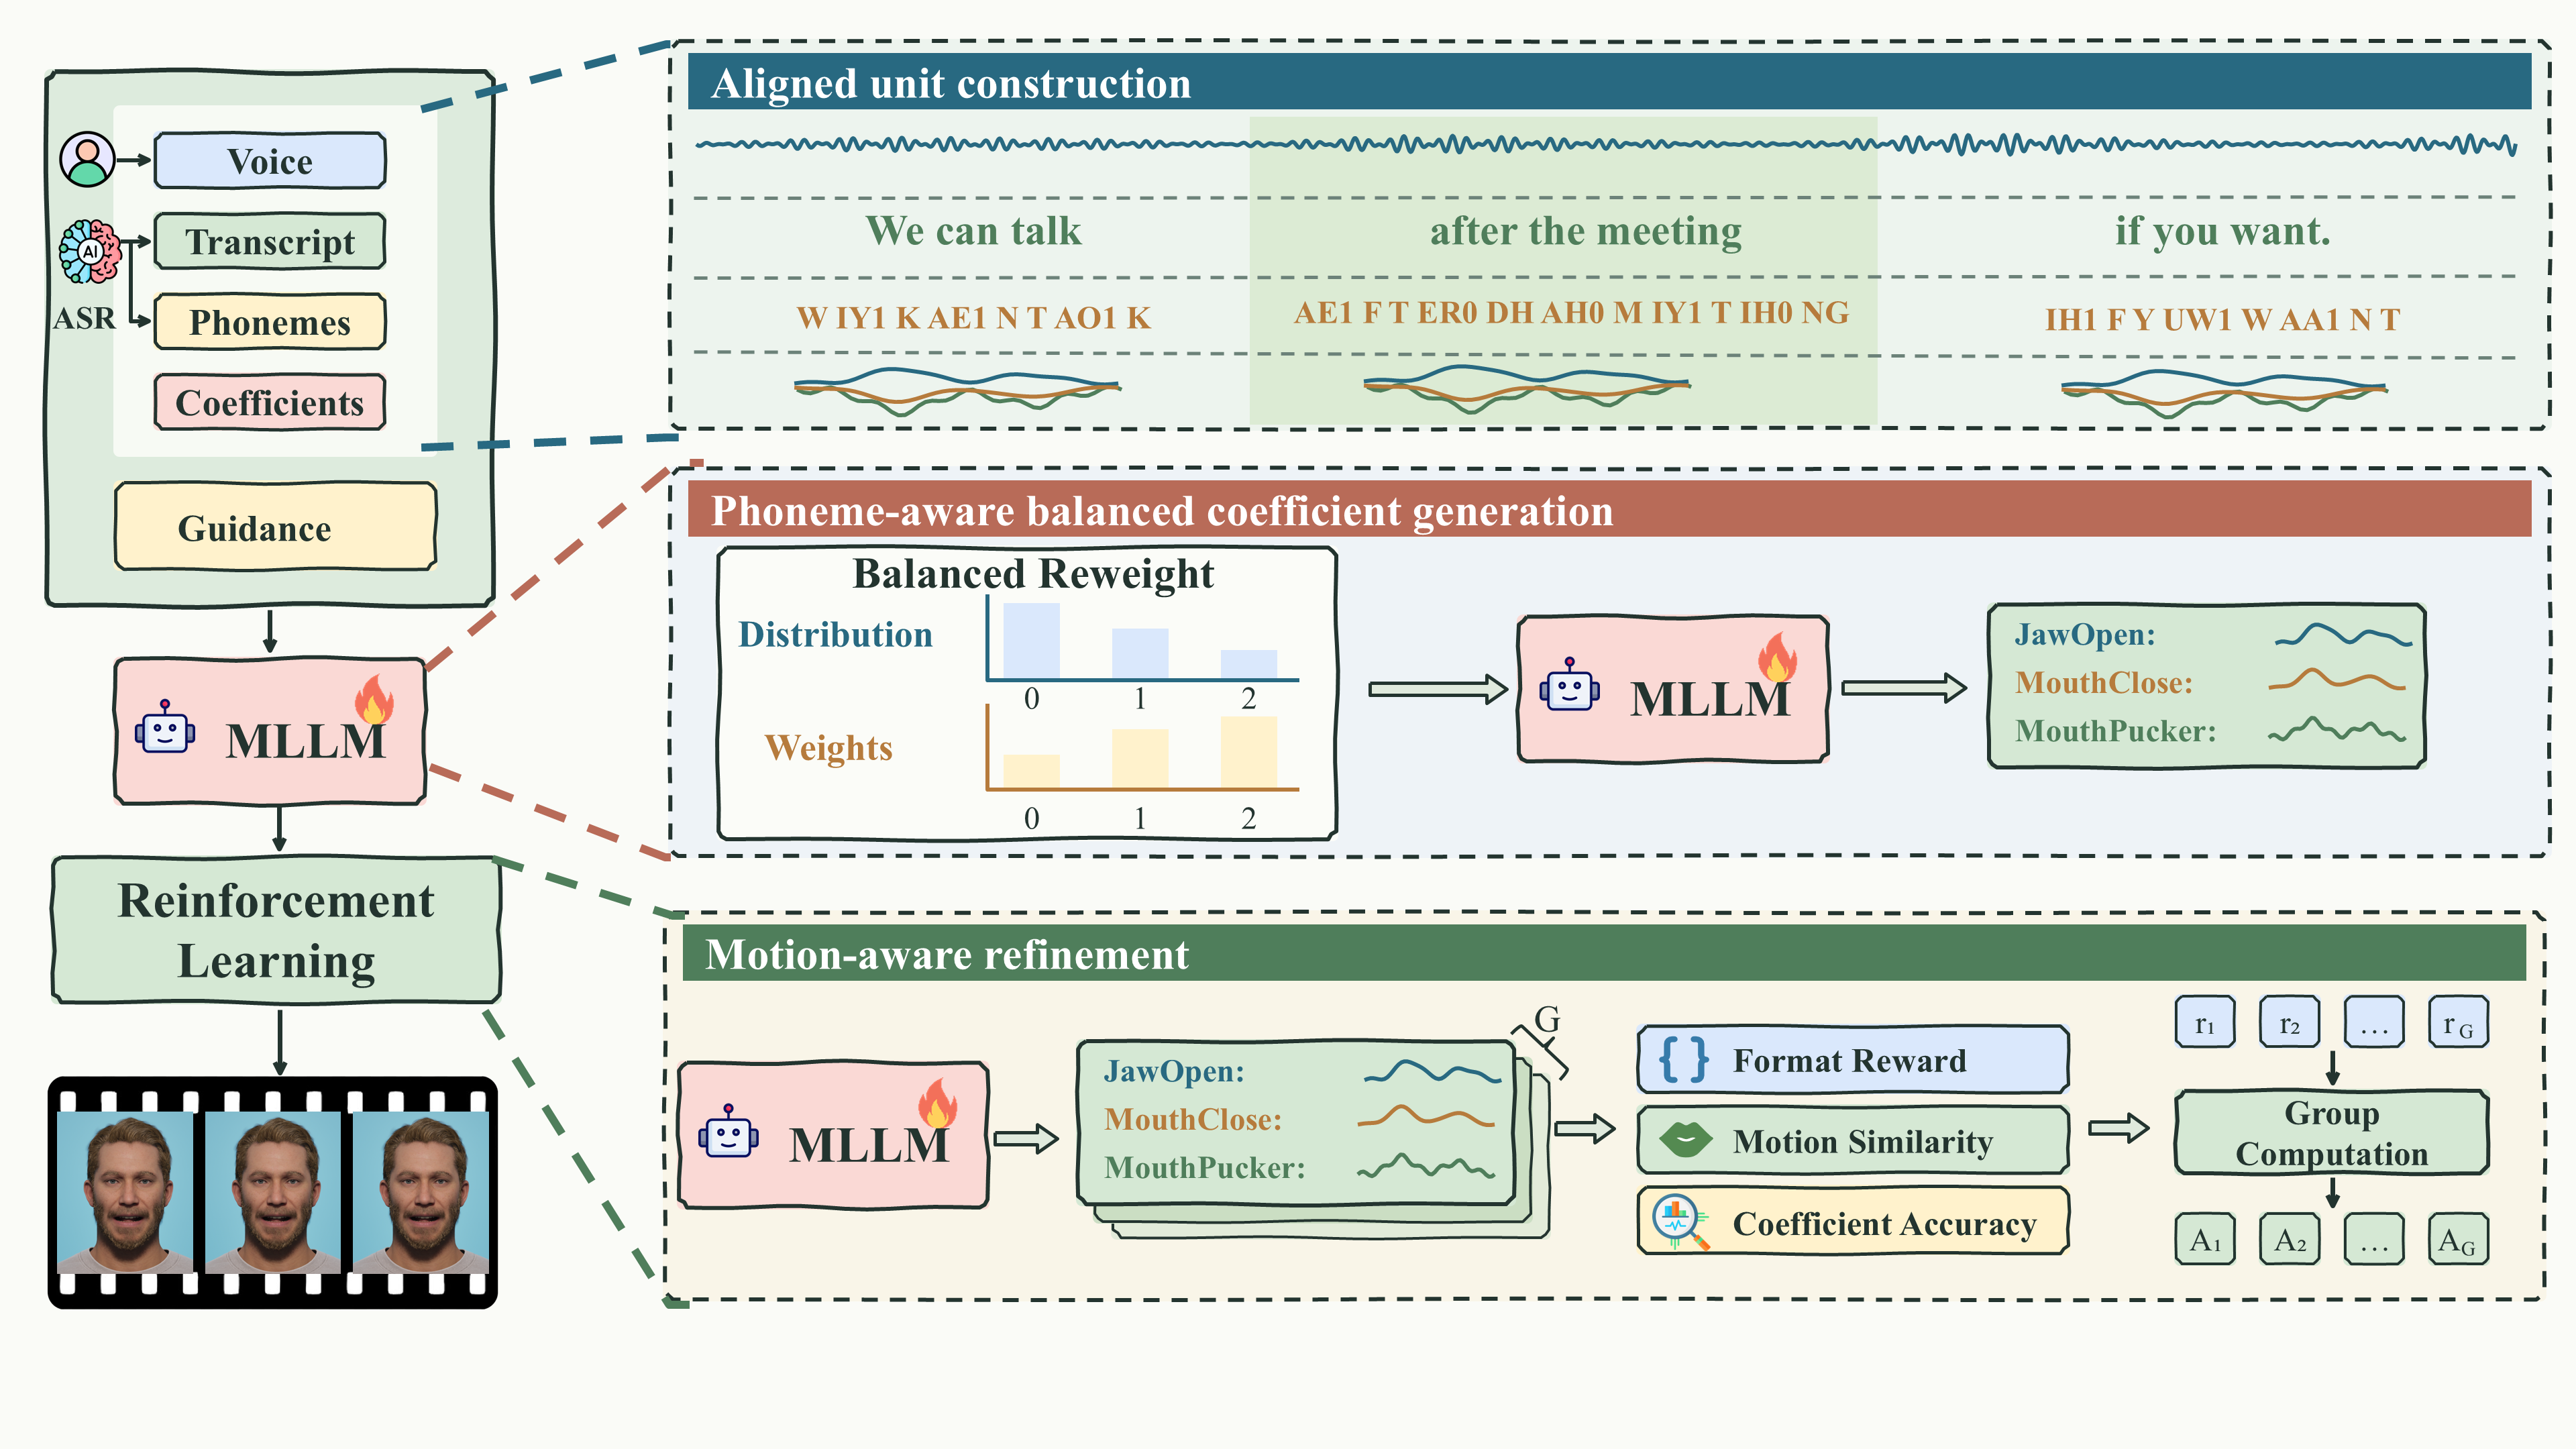
\includegraphics[width=0.80\textwidth]{img/method.png}
    \vspace{-2mm}
    \caption{AudioMouth makes articulation explicit at every stage. Aligned units tie each phoneme to the motion it produces (upper right), grounding and balanced supervision turn those phonemes into named facial controls (middle right), and a motion-level reward including 3D lip geometry corrects what token likelihood cannot measure (lower right).}
    \label{fig:overview}
    \vspace{-3mm}
\end{figure*}

\subsection{Structured Motion Generation}
\label{sec:formulation}

Given a speech waveform $\mathcal{A}\!=\!\{a_{n}\}_{n=1}^{N}$ of $N$ samples, our goal is to predict a synchronized coefficient sequence $\mathcal{V}\!=\!\{v_{t}\}_{t=1}^{T}$ over $T$ motion frames, where each $v_{t}\!\in\!\mathbb{R}^{K}$ holds the $K\!=\!32$ mouth-related ARKit controls~\citep{apple_arkit} retained by SAiD~\citep{park2023said}. We divide each recording into $J$ aligned units, so unit $j$ carries the inputs and target
\begin{gather}
    \mathcal{X}^{j}=\left(\mathcal{A}^{j},\,\mathcal{W}^{j},\,\mathcal{P}^{j},\,\mathcal{G}\right),\quad
    \mathcal{Y}^{j}=f_{\mathrm{json}}\!\left(\mathcal{V}^{j}\right), \label{eq:unit}
\end{gather}
where $\mathcal{W}^{j}$ and $\mathcal{P}^{j}$ are the transcript and phoneme sequence of the audio segment $\mathcal{A}^{j}$, $\mathcal{G}$ is the phoneme-to-articulation grounding of Sec.\ref{sec:stage2}, $\mathcal{V}^{j}$ is the target motion, and $f_{\mathrm{json}}(\cdot)$ serializes each ARKit channel into a predefined key holding that channel in temporal order. A fixed schema turns animation into generation without a regression head. The generator $f_{\mathrm{gen}}(\cdot)$ with parameters $\theta$ models $\mathcal{Y}^{j}\!=\!(y_{1},\cdots,y_{M_{j}})$ autoregressively as
\begin{gather}
    p_{\theta}\!\left(\mathcal{Y}^{j}\mid\mathcal{X}^{j}\right)=\prod_{m=1}^{M_{j}}p_{\theta}\!\left(y_{m}\mid y_{<m},\mathcal{X}^{j}\right), \label{eq:ar}
\end{gather}
where $M_{j}$ is the output length and $y_{<m}$ the preceding tokens. Two requirements follow, since conditioning only helps when it covers the same time span as the target, and the likelihood in Eq.(\ref{eq:ar}) is blind to the value distribution of the targets and to the shape of the decoded trajectory.

\subsection{Semantic-Aligned Audio-Linguistic Units}
\label{sec:stage1}

\noindent\textbf{Boundary-Shared Unit Construction.}\quad
To make a phoneme informative about motion, the phoneme and the motion must refer to the same interval, which a long recording does not supply. We therefore build units whose boundaries are shared by all four signals, using automatic speech recognition $f_{\mathrm{asr}}(\cdot)$~\citep{gao2023funasr,zhang2022paddlespeech} for the transcript and word-level timestamps $\tau$, and semantic segmentation $f_{\mathrm{seg}}(\cdot)$~\citep{frohmann2024segment} for coherent utterances,
\begin{gather}
    \left(\tilde{\mathcal{W}},\tau\right)=f_{\mathrm{asr}}\!\left(\mathcal{A}\right),\quad
    \left\{\mathcal{W}^{j}\right\}_{j=1}^{J}=f_{\mathrm{seg}}\!\left(\tilde{\mathcal{W}}\right). \label{eq:seg}
\end{gather}
The first and last words of $\mathcal{W}^{j}$ determine one interval through $\tau$, which selects $\mathcal{A}^{j}$, $\mathcal{P}^{j}$, and, during training, $\mathcal{V}^{j}$. Cutting at semantic boundaries instead of fixed-length windows keeps every unit a complete utterance, because a window that splits a word hands the generator a phoneme whose articulatory consequence lies outside the unit. At inference the same construction runs without the motion branch.

\subsection{Articulation-Grounded Balanced Generation}
\label{sec:stage2}

\noindent\textbf{Articulation Grounding.}\quad
Aligned phonemes tell the model when a speech sound occurs but not what the mouth does to produce it, and an audio-driven regressor has to recover that relation from motion data alone. AudioMouth instead states it. Specifically, the grounding $\mathcal{G}$ in Eq.(\ref{eq:unit}) is a fixed statement mapping phonetic categories to the named ARKit controls they drive, connecting bilabial consonants to lip closure and open vowels to larger jaw opening. Since the output schema reuses those control names, the model carries the relation from instruction to generated key instead of inferring it, while the audio stays responsible for how strongly each action is realized. We call this division \emph{articulation grounding}, and it is why phonemes and their meaning are supplied together.

\noindent\textbf{Distribution-Balanced Supervision.}\quad
Grounded conditioning still leaves the objective unbalanced, because most mouth channels are inactive at any instant and their near-zero values dominate the token stream. Under the plain likelihood of Eq.(\ref{eq:ar}) the model is rewarded most for predicting inactivity, so the large values that produce visible motion contribute a small fraction of the gradient. We therefore reweight the loss with a fixed function $\omega(\cdot)$ that downweights the frequent low-valued tokens, giving
\begin{gather}
    \mathcal{L}_{\mathrm{db}}=-\sum_{m=1}^{M_{j}}\omega\!\left(y_{m}\right)\log p_{\theta}\!\left(y_{m}\mid y_{<m},\mathcal{X}^{j}\right), \label{eq:db}
\end{gather}
where $\omega(y_{m})$ depends only on the value a coefficient token carries and equals one on every schema token, so keys and punctuation keep their weight and the output format is unaffected. The weighting is one monotone table, fixed before training and shared across all channels and all experiments, with values in Appendix~\ref{app:json}. Supervised fine-tuning with Eq.(\ref{eq:db}) yields $\theta_{\mathrm{sft}}$, which initializes refinement.

\subsection{Motion-Aware Refinement with Geometric Feedback}
\label{sec:stage3}

Even a well-balanced token objective scores a trajectory one value at a time, so it cannot separate a sequence that moves like the reference from one reaching similar values through implausible motion, and cannot tell which coefficient errors change the visible mouth. We close this gap by refining $\theta_{\mathrm{sft}}$ with Group Relative Policy Optimization (GRPO)~\citep{shao2024deepseekmath} against a reward computed on the decoded motion, where we sample $G$ candidates per input $\mathcal{X}^{j}$, parse each into a trajectory through $f_{\mathrm{parse}}(\cdot)$, and compare it with the reference $\mathcal{V}^{j}$.

\noindent\textbf{Simplified Lip-Geometry Discrepancy.}\quad
Coefficient-wise errors treat the $K$ controls as independent while the visible mouth is their joint result, so two candidates with equal coefficient error can differ greatly in shape, and rendering each candidate to measure that difference is far too slow inside a sampling loop. We therefore introduce the \emph{simplified lip-geometry discrepancy} (SLMD), which reads the shape difference out of the coefficients through a fixed blendshape basis. Let $\mathbf{C}^{p},\mathbf{C}^{g}\!\in\!\mathbb{R}^{T\times K}$ denote the candidate and reference sequences, and let $\mathbf{b}_{k,m}\!\in\!\mathbb{R}^{3}$ be the displacement the $k$-th blendshape applies to mouth-region vertex $m\!\in\!\mathcal{M}$ relative to the neutral mesh. Since both sequences are driven from the same neutral geometry, the neutral term cancels and the per-vertex displacement difference $\delta\mathbf{x}_{t,m}=f_{\mathrm{geo}}(\mathbf{C}^{p}\!-\!\mathbf{C}^{g})$ and the resulting discrepancy are
\begin{align}
    \delta\mathbf{x}_{t,m}&=\sum_{k=1}^{K}\left(c^{p}_{t,k}-c^{g}_{t,k}\right)\mathbf{b}_{k,m}, \label{eq:slmd_disp}\\
    \mathcal{L}_{\mathrm{slmd}}&=\frac{\sum_{t=1}^{T}\sum_{m\in\mathcal{M}}w_{m}\left\|\delta\mathbf{x}_{t,m}\right\|_{2}}{T\sum_{m\in\mathcal{M}}w_{m}}, \label{eq:slmd}
\end{align}
where the fixed vertex weights $w_{m}$ emphasize the lip region while retaining lower-weighted surrounding vertices, and $T$ is the compared length. SLMD therefore costs one matrix product per candidate, couples all $K$ controls through their shared effect on the surface, and stays in the coefficient domain, which keeps it independent of the rendered-video landmark metric used for evaluation.

\noindent\textbf{Motion-Level Reward.}\quad
Mouth quality involves both the shape at each instant and how that shape evolves, so SLMD alone is not sufficient. We combine it with the coefficient error $\mathcal{L}_{\mathrm{mse}}$ and the first- and second-order temporal difference discrepancies $\mathcal{L}_{\mathrm{vel}}$ and $\mathcal{L}_{\mathrm{acc}}$, which compare how the candidate changes against how the reference changes instead of penalizing movement itself. The four terms live on different numerical scales, so each is mapped to a bounded score before aggregation, giving
\begin{align}
    S_{q}=\left(1+\mathcal{L}_{q}/s_{q}\right)^{-1},\quad
    r_{\mathrm{motion}}=\sum_{q\in\mathcal{Q}}\lambda_{q}S_{q},\quad \mathcal{Q}=\left\{\mathrm{mse},\mathrm{vel},\mathrm{acc},\mathrm{slmd}\right\}, \label{eq:reward}
\end{align}
where each scale $s_{q}$ is the median of $\mathcal{L}_{q}$ measured once on reference data so the four scores occupy a comparable range, and the nonnegative weights $\lambda_{q}$ sum to one. Invalid schema instances receive a fixed negative reward and valid candidates of the wrong length are penalized in proportion to their length error, which keeps format compliance and duration control inside one signal. All scales, weights, and penalties are fixed once and reused across every experiment, with values in Appendix~\ref{app:refinement}.

\noindent\textbf{Group-Relative Policy Update.}\quad
To turn these absolute rewards into a learning signal without a value network, we normalize them within each sampled group as $\hat{A}_{i}=(r_{i}-\bar{r})/(\sigma_{r}+\epsilon)$, where $\bar{r}$ and $\sigma_{r}$ are the group mean and standard deviation and $\epsilon$ ensures numerical stability. Since all $G$ candidates answer the same input, the comparison isolates what the policy did differently on this utterance and favors the candidate whose motion is closer to the reference in shape and dynamics, so $\theta_{\mathrm{grpo}}$ keeps the schema learned during supervised fine-tuning and adds the sequence-level preference that token likelihood cannot express.

\noindent\textbf{Inference.}\quad
Given test speech, we build input units as in Sec.\ref{sec:stage1} and generate one coefficient JSON per unit with $\theta_{\mathrm{grpo}}$. The decoded segments are concatenated in temporal order and passed through $f_{\mathrm{post}}(\cdot)$, which suppresses residual jitter and the small discontinuities appearing where two independently generated units meet, giving
\begin{gather}
    \hat{\mathcal{V}}=f_{\mathrm{post}}\!\left(\mathrm{Concat}\!\left(\left\{f_{\mathrm{parse}}\!\left(\hat{\mathcal{Y}}^{j}\right)\right\}_{j=1}^{J}\right)\right). \label{eq:infer}
\end{gather}
Algorithm~\ref{alg:framework} summarizes the procedure, and Appendix~\ref{app:additional} verifies that $f_{\mathrm{post}}(\cdot)$ complements refinement instead of substituting for it.
